\documentclass[12pt, a4paper]{report}
\usepackage{graphicx} %LaTeX package to import graphics
\usepackage[shortlabels]{enumitem}
\usepackage{geometry}
\usepackage{xcolor}
\geometry{lmargin=30mm}
\usepackage[export]{adjustbox}
\usepackage{titlesec}
\usepackage{float}
\usepackage{listings}

\usepackage{hyperref}

\titleformat{\chapter}{\normalfont\huge}{\thechapter}{20pt}{\huge\bf}
\graphicspath{{images/}} %configuring the graphicx package
\title{Practica 5}
\author{Javier Izquierdo Hernández}
\date{\today}
\begin{document}
	\begin{titlepage}
		\centering
		{
\includegraphics[width=0.3\textwidth]{logo}\par}
		\vspace{1cm}
		{\bfseries\LARGE Universidad Rey Juan Carlos \par}
		\vspace{1cm}
		{\scshape\Large E.T.S. Ingeniería de Telecomunicación \par}
		\vspace{3cm}
		{\scshape\Huge Redes de Ordenadores para Robots y Máquinas Inteligentes \par}
		\vspace{3cm}
		{\itshape\Large Práctica 5\par}
		\vfill
		{\Large Autor: \par}
		{\Large Javier Izquierdo Hernández \par}
		\vfill
		{\Large \today \par}
	\end{titlepage}

\newpage
\renewcommand{\contentsname}{Contenidos}
\tableofcontents
\newpage

Para realizar esta práctica se necesita el emulador de redes Mininet-Wifi. Tienes 2 opciones:

\begin{enumerate}
	\item Puedes usar la máquina virtual mininet-wifi-ror.ova, que es una máquina Ubuntu con Mininet	Wifi ya instalado, preparada para importar directamente en VirtualBox.
	Puedes descargarla de: https://mobiquo.gsyc.urjc.es/mininet-wifi-ROR.ova
	Para entrar en el Ubuntu de la máquina virtual, el usuario es ’ror’ y la contraseña ’ROR20ROR’.
	\item Puedes instalar Mininet-Wifi en nativo en tu ordenador con Ubuntu con los siguientes comandos:
	\begin{center}
		sudo apt install git\\
		sudo apt install python-is-python3\\
		git clone https://github.com/intrig-unicamp/mininet-wifi\\
		cd mininet-wifi\\
		sudo util/install.sh -Wlnfv
	\end{center}
\end{enumerate}
Descarga tus escenarios de red para la práctica del siguiente enlace:

\begin{center}
https://mobiquo.gsyc.urjc.es/practicas/ror/p5.html
\end{center}

y descomprime el fichero lab-wifi.tgz.

\chapter{Escenario simple}
En el fichero escenario\_simple.py se encuentra definida una topología de red para Mininet Wifi.
Muévete a la carpeta donde has descomprimido el escenario lab-wifi y verás tres ficheros y una
captura. El escenario se arranca de la siguiente forma:
\begin{center}
	sudo ./escenario\_simple.py
\end{center}
El diagrama muestra las posiciones de cada uno de las estaciones y los APs. Fíjate en el alcance
que tienen ap1 y ap2 y piensa a qué APs estarán conectadas cada una de las 3 estaciones.
\begin{enumerate}
	\item Para saber qué interfaces de red tienen los APs y las estaciones, ejecuta el comando net desde la interfaz CLI y anota qué interfaces de red ha creado mininet-wifi para cada uno de los
	dispositivos.\\
	
	Se han creado las siguientes interfaces:
	\begin{figure}[h]
		\centering
		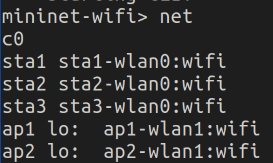
\includegraphics[width=0.8\textwidth]{ej1.1}
	\end{figure}
	\item Desde la interfaz CLI de mininet-wifi arranca un terminal para sta1 y desde ese terminal ejecuta
	el comando que muestra la configuración IP de esa estación y apunta la dirección MAC y dirección
	IP.\\
	
	La dirección MAC es la 00:00:00:00:09:11 y la IP es 11.209.0.1.
	\begin{figure}[h]
		\centering
		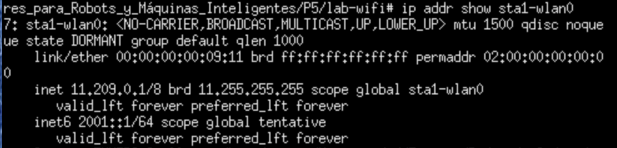
\includegraphics[width=0.8\textwidth]{ej1.2}
	\end{figure}
	\item Ejecuta el comando que muestra la información de la interfaz inalámbrica en sta1. Fíjate en la
	información sobre el modo de conexión, el SSID al que está conectado y el canal.\\
	
	El tipo de conexión es \textit{managed} y esta conectado al SSID de ssid1 y el canal es el 1.
	\begin{figure}[h]
		\centering
		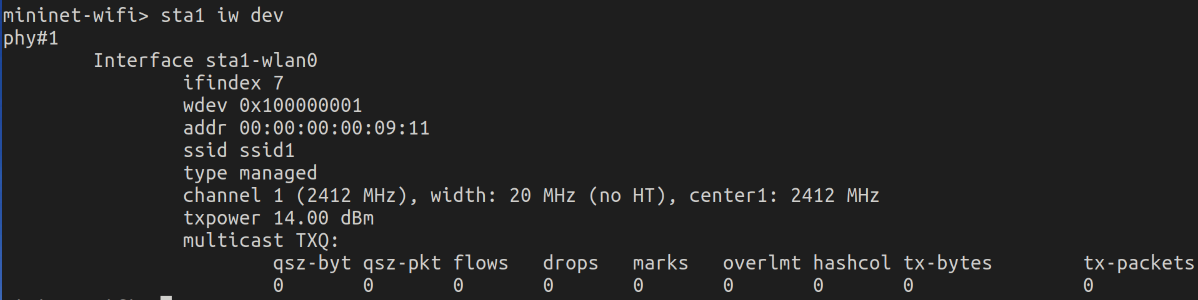
\includegraphics[width=0.8\textwidth]{ej1.3}
	\end{figure}
	\item Obtén la misma información de sta2, sta3 y realiza una tabla que resuma los datos de las 3
	estaciones:
	\begin{figure}[h]
		\centering
		\resizebox{\textwidth}{!}{\begin{tabular}{ |c|c|c|c|c|c|c| } 
			\hline
			Dispositivo & Interfaz inalámbrica & Dir. MAC & Dir. IP &Tipo de conexión & SSID & Canal\\
			\hline
			sta1 & sta1-wlan0 & 00:00:00:00:09:11 & 11.209.0.1 & managed & ssid1 & 1 (2412 MHz), width: 20 MHz (no HT), center1: 2412 MHz\\ 
			\hline
			sta2 & sta2-wlan0 & 00:00:00:00:09:22 & 11.209.0.2 & managed & ssid1 & 1 (2412 MHz), width: 20 MHz (no HT), center1: 2412 MHz\\
			\hline
			sta3 & sta3-wlan0 & 00:00:00:00:09:33 & 11.209.0.3 & managed & ssid2 & 10 (2457 MHz), width: 20 MHz (no HT), center1: 2457 MHz\\
			\hline
		\end{tabular}}
	\end{figure}
	\item Como sta1 y sta2 están asociadas al mismo AP hay conectividad entre ambas estaciones, pero
	no hay conectividad con sta3 porque no se ha configurado una red que conecte ambos AP. Para
	comprobarlo lanza wireshark en sta1 (lo puedes lanzar en background o crear otro terminal para
	sta1) y selecciona la interfaz inalámbrica de sta1. A continuación ejecuta un ping para que
	envíe 3 paquetes a sta2 y después otro ping para que envíe 3 paquetes a sta3. Interrumpe la
	captura y guarda su contenido en el fichero \textcolor{blue}{wifi-01.cap}. Explica en la memoria el contenido de
	la captura.
\end{enumerate}

En los mensajes capturados verás que las cabeceras que aparecen en el nivel de enlace tienen el
formato de mensajes Ethernet, y no se muestran las cabceras del protocolo 802.11. Normalmente los
drivers de las tarjetas inalámbricas transforman el paquete 802.11 en formato 802.3 (Ethernet). Para
poder analizar el tráfico 802.11 es necesario hacer uso de una interfaz especial que crea mininet-wifi
para procesar el tráfico inalámbrico.\\

Desde la máquina real ejecuta:
\begin{center}
	\textbf{sudo ifconfig hwsim0 up}
\end{center}
Lanza Wireshark seleccionado esta interfaz para realizar la captura. En esta interfaz se pueden
capturar todos los mensajes de ap1 y ap2. Vamos a provocar una nueva asociación de sta1 a ap1 para
ver todos los mensajes 802.11.\\

Desconecta sta1 de la red ssid1 que es en la que se encuentra asociada y verifica que ya no está
asociada a dicha red.\\

Ahora reconectaremos la estación a ap1 y capturaremos los mensajes intercambiado en el proceso
de la asociación.\\

Después de pocos segundos verás como la estación y el AP han intercambiado mensajes. Interrumpe
la captura y guarda el contenido en un fichero \textcolor{blue}{wifi-02.cap}.\\

En la captura verás como los mensajes además de la cabecera 802.11 tienen más información que
no forma parte de la trama 802.11. Son metadatos que llevan información del nivel físico y que pueden
ser datos importantes para analizar la capturas: Radiotap header y 802.11 Radio information.\\

Analiza la captura:
\begin{enumerate}
	\setcounter{enumi}{5}
	\item Selecciona un mensaje de baliza enviado por el ap1, dirección Ethernet de origen 00:00:00:00:00:01:
	\begin{enumerate}[label=\alph*)]
		\item Indica qué canal está utilizando para transmitir, la tasa de envío y la frecuencia utilizada.\\
		
		Esta usando el canal 1, la tasa de envío es de 1 Mb/s y la frecuencia es de 2412 MHz.
		\item Indica los valores de los bits To Ds y From DS que viajan en el campo Flags del campo
		Control Field:\\
		\begin{itemize}
			\item To DS: 0
			\item From DS: 0
		\end{itemize}
		\item Teniendo en cuenta los valores anteriores, indica los valores de las 3 direcciones MAC que
		lleva la trama baliza y explica a qué máquinas corresponden. Comprueba en la interfaz
		hexadecimal de wireshark que las 3 direcciones van una a continuación de la otra, después
		está el número de secuencia (2 bytes) y que detrás no hay un campo para la 4ª dirección.\\
		
		Las 3 direcciones MAC son:
		\begin{itemize}
			\item Receiver/Destination: ff:ff:ff:ff:ff:ff\\
			\item Transmiter/Source: 00:00:00:00:09:01\\
			\item BSS Id: 00:00:00:00:09:01 \\
		\end{itemize}
		Si que se cumple que después de la tercera dirección MAC esta el numero de secuencia que esta vacio.
		\item ¿Por qué crees que el número de secuencia de una trama baliza es siempre 0?\\
		
		Porque sirve para indicar a los nuevos dispositivos que hay se encuentra un Ap, es decir, inicia la conversación con una estación, por eso es 0.
		\item Indica cuál es el intervalo entre tramas baliza\\
		
		El intervalo es 0,1024 segundos.
		\item Indica cuál es el SSID que se está usando.\\
		
		Se esta usando el ssid1.
		\item Busca en el campo Capabilities algún campo que indique que el dispositivo que está
		transmitiendo es un AP.\\
		
		El primer apartado del campo Capabilities llamado ESS Capabilities indica que el dispositivo es un AP.
	\end{enumerate}
	\item Selecciona el primer mensaje Probe Request de sta1:
	\begin{enumerate}[label=\alph*)]
		\item Explica los valores del campo To DS y From DS y las 3 direcciones y a qué máquinas se
		refiere.\\
		
		Los valores de To Ds y From DS son 0 y 0, ya que lo envía al broadcast. Y las 3 direcciones MAC son:
		\begin{itemize}
			\item Receiver/Destination: ff:ff:ff:ff:ff:ff\\
			\item Transmiter/Source: 00:00:00:00:09:11; Se refiere a sta1.\\
			\item BSS Id: ff:ff:ff:ff:ff:ff \\
		\end{itemize}
		\item Fíjate si el mensaje Probe Request lleva en alguna cabecera el SSID al que se quiere conectar
		y el canal.\\
		
		Lleva el SSID en la cabecera de Wireless Management y este es el de ssid1, pero no se especifica el canal exacto en el que se quiere conectar, sino que se especifican los canales soportados.
		\item ¿Por qué crees que hay varios mensajes Probe Request?\\
		
		Porque estos mensajes se envían por todos los canales para encontrar el mejor Ap.
	\end{enumerate}
	\item Selecciona el mensaje Probe Response:
	\begin{enumerate}[label=\alph*)]
		\item Explica qué valores tienen los posibles 4 campos de direcciones y a qué máquinas se refiere.\\
		
		Como los campos To Ds y From Ds son 0 y 0 entonces solo habrá 3 direcciones MAC.
		
		\begin{itemize}
			\item Receiver/Destination: 00:00:00:00:09:11; Se refiere a sta1.\\
			\item Transmiter/Source: 00:00:00:00:09:11; Se refiere a ap1.\\
			\item BSS Id: 00:00:00:00:09:11; Se refiere a ap1. \\
		\end{itemize}
		\item Indica qué campo muestra el canal en el que el AP está realizando la respuesta.\\
		
		Se encuentra en el campo 802.11 radio information. Y dentro de este campo en el apartado channel.
		\item Indica qué campo muestra el SSID que está usando el AP.\\
		
		El Ap esta usando ssid1.
	\end{enumerate}
	\item Fíjate que después del mensaje Probe Response hay un asentimiento dirigido a ap1 para confirmar la recepción de Probe Response. Observa que los asentimientos en wifi no indican el
	número de secuencia que se asiente, por lo que asienten la última trama recibida, y el emisor
	no enviará otra trama hasta tener asentida la anterior. ¿Cuántas direcciones lleva el mensaje de
	asentimiento?\\
	
	El mensaje de asentimiento solo lleva 1 dirección MAC que es la de ap1 \textit{(Receiver: 00:00:00:00:09:01)}.
	\item Selecciona el mensaje Authentication que envía la estación:
	\begin{enumerate}[label=\alph*)]
		\item En la asociación no están usando autenticación, indica donde se muestra esta información y
		el número de secuencia asociado a la fase de autenticación, fíjate que es diferente del número
		de secuencia de la cabecera general de 802.11 (Sequence Number).\\
		
		Esta información se muestra en el campo de Wireless Management, en el apartado de \textit{Fixed Parameters}.
		El número de secuencia asociado a la autenticación es \textbf{0x0001}, mientras que el global es de 29.
	\end{enumerate}
	\item Selecciona el mensaje Authentication que envía el AP:
	\begin{enumerate}[label=\alph*)]
		\item Comprueba que lleva el mismo algoritmo de autenticación que la solicitud y comprueba el
		número de secuencia asociado a la fase de autenticación.\\
		
		El algoritmo de autenticación es el mismo, que es \textit{Open System}, y el número de secuencia es el siguiente (\textbf{0x0002}).
		\item Observa que ambos mensajes de autenticación están asentidos, fíjate que sólo se distinguen
		por la dirección destino.
		\begin{figure}[h]
			\centering
			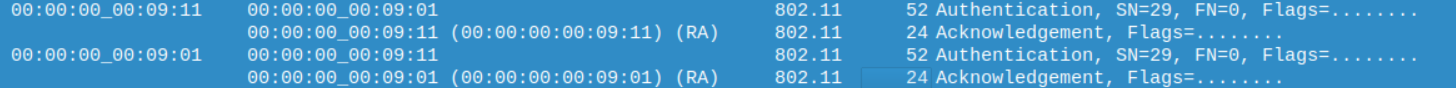
\includegraphics[width=0.8\textwidth]{ej1.11}
		\end{figure}
	\end{enumerate}
	\item Comprueba en el mensaje Association Request que viaja el SSID y el Listen Interval. Recuerda
	que el Listen Interval está expresado en número de intervalos de envío de tramas baliza. Además
	comprueba que el número de secuencia de la cabecera general de 802.11 es uno más que el del
	mensaje de autenticación enviado por sta1.\\
	
	El SSID es ssid1 y el Listen Interval es de \textbf{0x0005}.\\
	Y podemos comprobar que el número de secuencia es 1 mayor que es 30.
	\item Identifica el AID (Association ID) que viaja en el mensaje Association Response. Y comprueba
	que el número de secuencia de la cabecera general de 802.11 es uno más que el del mensaje anterior
	enviado desde ap1.\\
	
	El AID es \textbf{0x0001} y en efecto el número de secuencia es de 1 más que es 30.
	\item Desde el terminal de la estación sta1 realiza un escaneo para ver que redes inalámbricas son
	visibles desde ese punto y realiza lo mismo desde sta2 y sta3 (el escaneo tarda unos segundos).
	Anota la potencia de señal recibida de cada AP.\\
	\begin{itemize}
		\item Desde sta1 se conecta con Ap1 con una potencia de -76,00 dB\\
		\item Desde sta2 se conecta con Ap1 con una potencia de -86,00 dB\\		
		\item Desde sta2 se conecta con Ap2 con una potencia de -90,00 dB\\
		\item Desde sta3 se conecta con Ap2 con una potencia de -86,00 dB\\
	\end{itemize}
	
	\begin{figure}[H]
		\centering
		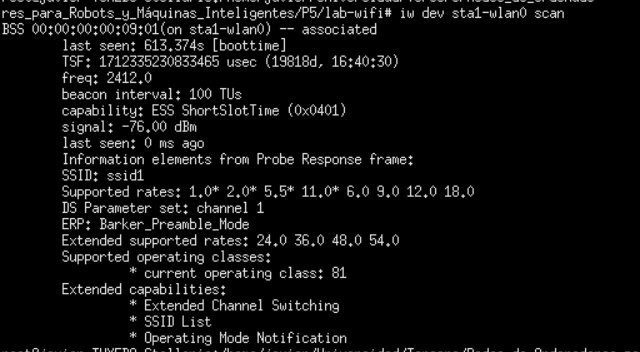
\includegraphics[width=0.8\textwidth]{ej1.14_1}
	\end{figure}
	\begin{figure}[H]
		\centering
		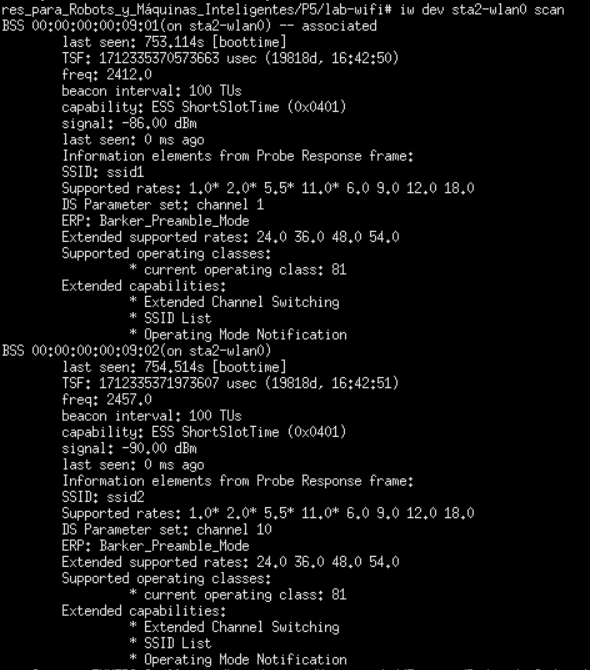
\includegraphics[width=0.8\textwidth]{ej1.14_2}
	\end{figure}	
	\begin{figure}[H]
		\centering
		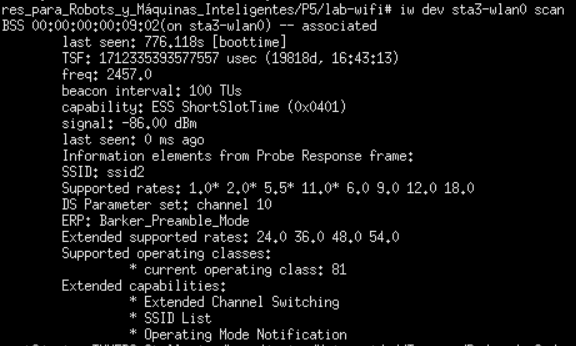
\includegraphics[width=0.8\textwidth]{ej1.14_3}
	\end{figure}
	\item Para saber la distancia desde cada AP a las estaciones ejecuta el siguiente comando en la interfaz
	CLI mininet-wifi, por ejemplo para ver la distancia entre sta1 y ap1:
	\begin{center}
		\textbf{mininet-wifi$>$ distance sta1 ap1}
	\end{center}
	Compara estas distancias de cada estación con los AP con los que tiene visibilidad y con la
	potencia de señal recibida en cada estación.\\
	\begin{figure}[H]
		\centering
		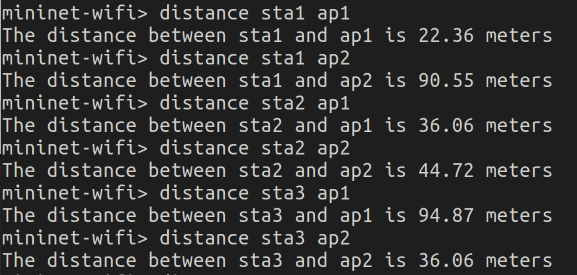
\includegraphics[width=0.8\textwidth]{ej1.15}
	\end{figure}
	Sta1 solo tiene visible a ap1, ya que ap2 esta a más de 90 metros. Y como es la estación que tiene a menor distancia un ap, en este caso ap1, es la que menor potencia recibe (Es mejor cuanto menos potencia).
	
	En el caso de Sta2 tiene visibles a ambos Ap, ya que la distancia a ambos es menor de 50 metros, y por lo tanto la potencia de la señal será mayor que con sta1.
	
	Y por último con Sta3, esta solo ve a Ap2, ya que Ap1 está muy lejos, y la señal de Sta3 a Ap2 es igual a la de Sta2 a Ap1 ya que están a la misma distancia.
	\item Con el siguiente comando vamos a mover a sta1 a otra coordenada fuera del alcance de cualquier
	AP y sta. Elige tú la coordenada (X,Y) y ejecuta lo siguiente en la interfaz CLI de mininet-wifi:
	\begin{center}
		\textbf{py sta1.setPosition('X,Y,0')}
	\end{center}
	Comprueba la nueva posición en el dibujo. Y ejecuta un escaneado para ver que ya no tiene
	alcance a ningún AP y estación.
	\begin{figure}[H]
		\centering
		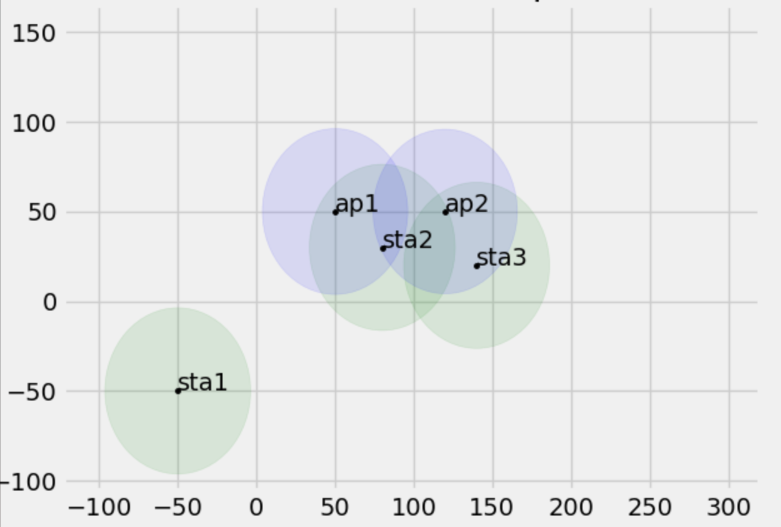
\includegraphics[width=0.8\textwidth]{ej1.16_1}
	\end{figure}
	Como se puede ver en la imagen, ahora sta1 no encuentra ningún Ap.
	\begin{figure}[H]
		\centering
		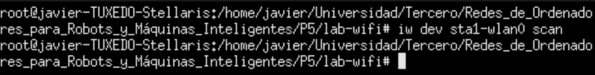
\includegraphics[width=0.8\textwidth]{ej1.16_2}
	\end{figure}
	\item Mueve la estación sta1 a esta nueva posición (120,20,0), fíjate en la figura que muestra mininet-wifi y comprueba desde el terminal de sta1 que se ha asociado con ap2. También comprueba que
	ahora puede comunicarse con sta3 pero no con sta2 ya que ahora sta1 estará asociada a ap2
	(al igual que sta3). Y aunque sta2 podría estar asociada a ap2 porque se encuentra en su radio
	de acción, sta2 está asociada a ap1 por recibir su señal con una potencia algo mayor.\\
	
	En la imagen inferior se puede ver que sta1 solo encuentra ap2.
	\begin{figure}[H]
		\centering
		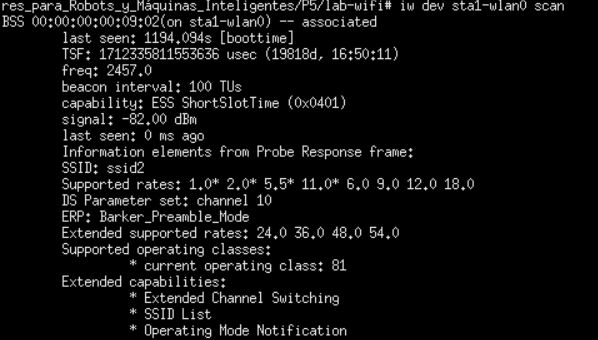
\includegraphics[width=0.8\textwidth]{ej1.17_1}
	\end{figure}
	Como se puede ver en la imagen, ahora sta1 no es capaz de comunicarse con sta2, pero si con sta3.
	\begin{figure}[H]
		\centering
		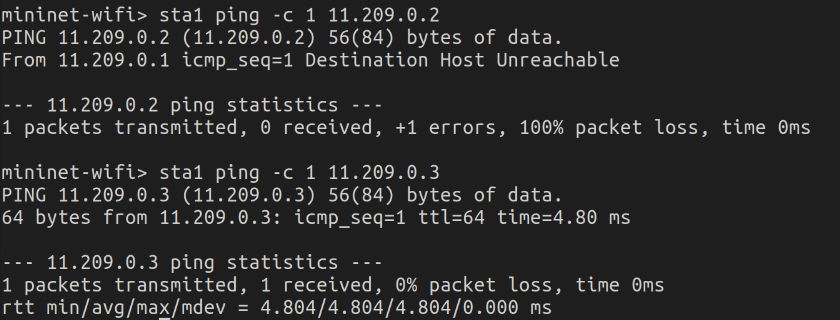
\includegraphics[width=0.8\textwidth]{ej1.17_2}
	\end{figure}
	\item Lanza una nueva captura en la interfaz hwsim0 y realiza desde sta1 un ping -c 3 a sta3. Una
	vez terminada la ejecución del ping interrumpe la captura y guárdala en el fichero \textcolor{blue}{wifi-03.cap}.
	Analiza el contenido y explica los mensajes que son consecuencia de la ejecución del ping:
	\begin{enumerate}[label=\alph*)]
		\item ¿Cuántos mensajes ICMP echo request hay? ¿Y cuántos ICMP echo reply? ¿Por qué?\\
		
		Hay 6 ICMP echo request y 6 ICMP echo reply porque se envian desde sta1 a ap2 y desde ap2 a sta3 en ambos sentidos.
		\item Fíjate en las direcciones que llevan estos mensajes y justifica sus valores.\\
		
		En los mensajes request de sta1 a ap2 las direcciones son:
		\begin{itemize}
			\item Receiver/BSS Id: 00:00:00:00:09:02; El Ap al que va el mensaje es Ap2\\
			\item Transmiter/Source: 00:00:00:00:09:11; La estación de origen es sta1\\
			\item Destination: 00:00:00:00:09:33; La estación de destino del ping que es sta3\\
			\item STA address: 00:00:00:00:09:11; La estación de origen es sta1\\
		\end{itemize}
		En los mensajes request de ap2 a sta3 las direcciones son:
		\begin{itemize}
			\item Receiver/Destination: 00:00:00:00:09:33; La Sta a la que va el mensaje es sta3\\
			\item Transmiter/BSS Id: 00:00:00:00:09:02; El ap que reenvia el ping es Ap2\\
			\item Source: 00:00:00:00:09:11; La estación de origen del ping que es sta1\\
			\item STA address: 00:00:00:00:09:11; La estación de destino es sta3\\
		\end{itemize}
		En los mensajes reply de sta3 a ap2 las direcciones son:
		\begin{itemize}
			\item Receiver/BSS Id: 00:00:00:00:09:02; El Ap al que va el mensaje es Ap2\\
			\item Transmiter/Source: 00:00:00:00:09:33; La estación de origen es sta3\\
			\item Destination: 00:00:00:00:09:11; La estación de destino del ping que es sta1\\
			\item STA address: 00:00:00:00:09:33; La estación de origen es sta3\\
		\end{itemize}
		En los mensajes reply de ap2 a sta1 las direcciones son:
		\begin{itemize}
			\item Receiver/Destination: 00:00:00:00:09:11; La Sta a la que va el mensaje es sta1\\
			\item Transmiter/BSS Id: 00:00:00:00:09:02; El ap que reenvia el ping es Ap2\\
			\item Source: 00:00:00:00:09:33; La estación de origen del ping que es sta3\\
			\item STA address: 00:00:00:00:09:11; La estación de destino es sta1\\
		\end{itemize}
		\item Observa los mensajes de asentimiento. Explica qué mensaje asiente cada asentimiento.\\
		
		El primero asiente que el mensaje ha llegado desde sta1 a Ap2, el segundo que ha llegado a sta3 desde Ap2. El tercero asiente que el mensaje a pasado de sta3 a Ap2, y por último se asiente para indicar que el mensaje a llegado a sta1 desde Ap2.
	\end{enumerate}
\end{enumerate}
\chapter{Tramas RTS/CTS}
Dentro del entorno de simulación mininet-wifi no se envían nunca utilizando tramas RTS/CTS
(Request to Send, Clear to Send). Para ver estas tramas carga el fichero de captura rts-cts.cap en
Wireshark.
\begin{enumerate}
	\item Observa los mensajes 1 y 2 e indica la dirección MAC de la estación que tiene datos que enviar
	y la dirección MAC de la estación que está concediendo el permiso.\\
	
	La dirección MAC de la estación que tiene datos que enviar es 90:8d:6c:ac:8b:b1, y la de la que concede el permiso es 68:f9:56:57:cc:97.
	\item ¿Cuál es el mensaje que lleva los datos?\\
	
	Es el tercer mensaje.
	\item En el mensaje 3 observa la cabecera IEEE 802.11, en la pestaña Flags, indica si se puede saber
	que el nodo que está transmitiendo es un AP o una estación, y si los datos están protegidos
	(cifrados). Observa que si los datos fueran en claro, se podrían examinar las siguientes cabeceras
	de la pila TCP/IP, cosa que aquí no sucede.\\
	
	Se puede saber que el nodo que transmite es una estación y que los datos están cifrados o protegidos.
	\item El mensaje 4 es un asentimiento de un conjunto de datos Block ACK. Dentro de la pestaña
	Compressed BlockAck Response va codificado el conjunto de tramas que asiente.
	El Block Ack Bitmap es un campo donde cada bit representa si se ha recibido ACK (1) o no se
	ha recibido (0) una trama concreta. Con los 8 bytes de este campo (64 bits) se pueden identificar
	64 tramas, es decir, se puede indicar si se ha recibido o no 64 números de secuencia comenzando
	en el número de secuencia especificado en Starting Sequence Number. A la vista de este campo,
	indica qué número/s de secuencia se están asintiendo.\\
	
	Solo se asiente el mensaje con el número de secuencia 8.
	\item Analiza el campo Duration de los mensajes 1, 2, 3 y 4.\\
	\begin{itemize}
		\item Mensaje 1: Duration: $28\mu s$\\
		\item Mensaje 2: Duration: $28\mu s$\\
		\item Mensaje 3: Duration: $48\mu s$\\
		\item Mensaje 4: Duration: $32\mu s$\\
	\end{itemize}
	\item Los mensajes 5 y 7 no llevan datos, indican respectivamente que el dispositivo se va a suspender
	(modo de baja energía) y se va a despertar. Despliega la pestaña Flags e indica la diferencia que
	ves entre ellos.\\
	
	La única diferencia es que el campo de PWR MGT esta a 1 en el mensaje 5 (La estación se va a dormir) y en el 7 esta a 0 (La estación se mantiene despierta).
\end{enumerate}
\chapter{Autenticación}
Arranca el escenario:
\begin{center}
	\textbf{sudo ./authentication.py}
\end{center}
\begin{enumerate}
	\item Desde la interfaz mininet-wifi$>$ puedes ver la configuración de red que se ha arrancado, para ello
	ejecutamos el comando dump. Anota las interfaces y direcciones IP de cada dispositivo. Deberías
	identificar 2 estaciones y un AP.\\
	
	Las direcciones Ip son las que se ven en la imagen inferior.
	\begin{figure}[H]
		\centering
		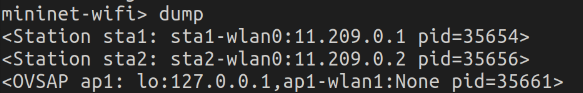
\includegraphics[width=0.8\textwidth]{ej3.1}
	\end{figure}
	\item Consulta a qué SSID están asociados sta1 y sta2.\\
	
	Tanto sta1 como sta2 no están asociados a ningún ssid.
	\begin{figure}[H]
		\centering
		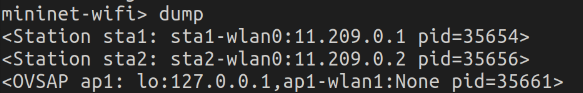
\includegraphics[width=0.8\textwidth]{ej3.1}
	\end{figure}
	\item Activa la interfaz hwsim0 y lanza una captura. Los nodos sta1 y sta2 ya han realizado la fase
	de asociación con el AP. Para ver el proceso de intercambio inicial de los mensajes entre una
	estación y el AP vamos a desconectar y conectar la interfaz inalámbrica de sta1:
	\begin{center}
		\textbf{ifconfig sta1-wlan0 down\\
			ifconfig sta1-wlan0 up}
	\end{center}
	A los pocos segundos observarás que se han intercambiado mensajes para la autenticación y
	asociación de sta1. Interrumpe la captura y guarda el contenido en el fichero \textcolor{blue}{wifi-04.cap}.\\
	
	Selecciona el mensaje Authentication que envía la estación. ¿Qué algoritmo de autenticación se
	está usando?\\
	
	Esta usando Open System.
	\item Identifica los 4 mensajes para el intercambio de información de claves. Explica qué tipo de trama
	802.11 tienen estos mensajes y su estructura de cabeceras. En particular, indica para qué sirve
	el campo Type de la cabecera LLC y que valor lleva.\\
	
	Los mensajes para el intercambio de claves son los siguientes:
	\begin{figure}[H]
		\centering
		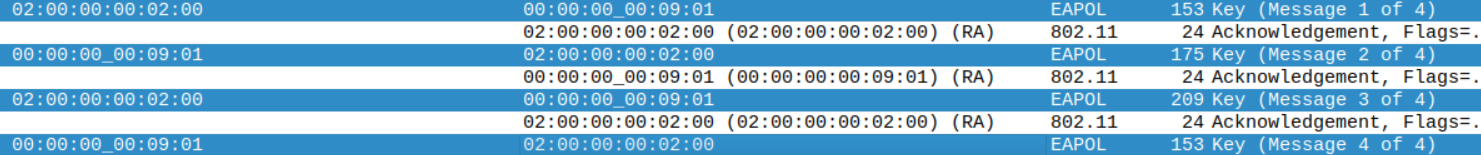
\includegraphics[width=0.8\textwidth]{ej3.4}\\
	\end{figure}
	Estos mensajes tienen un tipo de trama 802.1X Authentication en el que proveen de toda la información necesaria para realizar el intercambio de claves. El campo Type sirve para indicar que el tipo de la siguente cabecera es el dicho anteriormente.
	\item Para cada uno de esos 4 mensajes, identifica los campos importantes que deberían llevar y anota
	sus valores: ANonce, SNonce y direcciones MAC de los dos nodos. Recuerda que a partir de esta
	información y el secreto compartido a priori (“clave de la wifi”) se derivarán las claves que se
	usarán en la sesión para cifrar los mensajes.\\
	
	Las direcciones MAC de los nodos siempre son 02:00:00:00:02:00 y 00:00:00:00:09:01, y los valores de ANonce (mensajes 1 y 3) y SNonce (2 y 4) son los siguientes:
	\begin{itemize}
		\item ANonce: 46492804fd65426483b1c2662d0279f1c79ec0f52cd7f5f302324dd91a7c12ad\\
		\item SNonce: 4d0677d2383dc3f267464dcb770a1b5c38a4696d9831025f40057d573c72dc6c
	\end{itemize}
	
	\item Verás a continuación algún mensaje dirigido a alguna dirección especial de IPv6 pero si seleccionas el mensaje no puedes ver su contenido. Es necesario descifrarlo. Selecciona en el menú
	de Wireshark “Visualización” → “Barra de herramientas de Wireless”. En la nueva barra que
	ha aparecido en la interfaz, selecciona “Preferencias de 802.11” → “Decryption keys” → “Edit”
	e introduce un algoritmo con “Key Type” wpa-pwd y clave 123456789a. Guarda los cambios y
	observarás que los mensajes de IPv6 se han descifrado pudiendo acceder a todas sus cabeceras.
	Explica qué tipo de trama 802.11 es este paquete IPv6, y qué tipo de paquete IPv6.\\
	
	Recuerda: para poder descifrar el tráfico 802.11 más allá de la cabecera 802.11 es necesario tener
	en la captura los mensajes de intercambio de claves (4-way-handshake) y conocer la clave de la
	wifi. A partir de esta información se pueden calcular las claves de sesión y descifrar el tráfico.\\
		
	Es una trama de tipo Data y el paquete es de tipo ICMPv6.
\end{enumerate}
\chapter{Red ad-hoc}
En el modo ad-hoc no hay AP, y las estaciones se conectan entre ellas a un SSID y canal común.
Arranca el escenario para analizar este modo de funcionamiento:
\begin{center}
	\textbf{sudo ./simple\_adhoc.py}
\end{center}
\begin{enumerate}
	\item Extrae la información de las direcciones IP de cada una de las estaciones y el SSID y canal que
	están usando.\\
	
	La dirección Ip de sta1 es 11.209.0.1, de sta2 es 11.209.0.2 y de sta3 es 11.209.0.3, y el SSID y el canal se pueden ver en las siguientes imágenes.
	\begin{figure}[H]
		\centering
		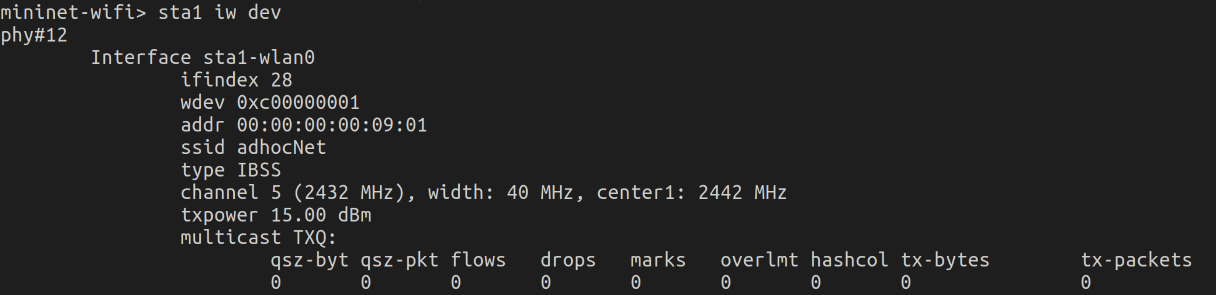
\includegraphics[width=0.8\textwidth]{ej4.1_1}\\
		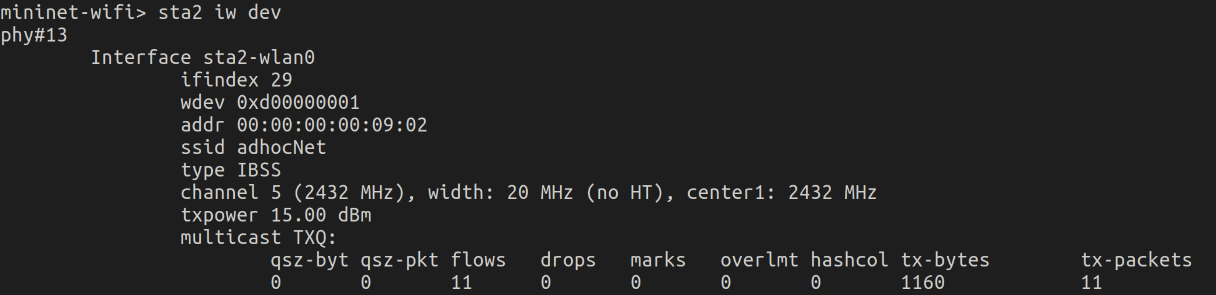
\includegraphics[width=0.8\textwidth]{ej4.1_2}\\
		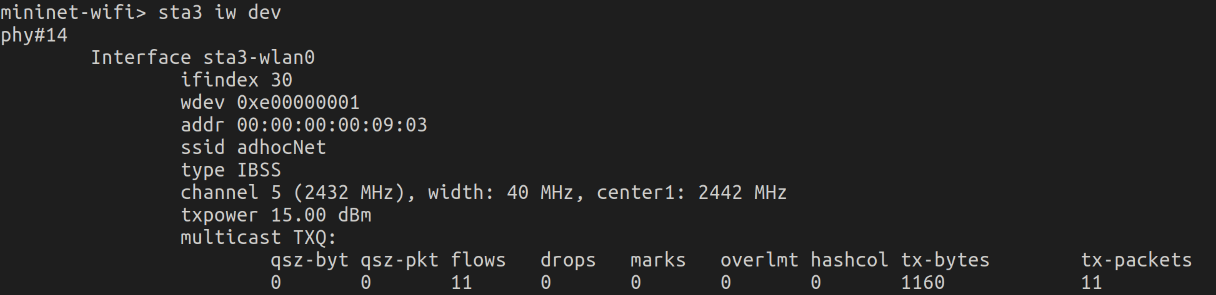
\includegraphics[width=0.8\textwidth]{ej4.1_3}
	\end{figure}
	\item Activa la interfaz hwsim0 y realiza una captura. Indica qué estación o estaciones están enviando
	tramas beacon.\\
	
	Todas las estaciones están enviando tramas \textit{Beacon}.
	\item Mientras está capturando wireshark, ejecuta una prueba de ping entre todas las estaciones. Interrumpe la captura y guarda su contenido en el fichero \textcolor{blue}{wifi-05.cap}. Explica los resultados
	obtenidos.\\
	
	En la captura se ve que las tres estaciones están enviado tramas \textit{beacon} y que cuando se ejecutan los ping estos se envían como si fueran por cable salvo por los mensajes de Acknowledge. La única excepción es que no se hace ping de sta1 a sta3, ya que al estar en modo adHoc y no estar en rango una de otra no se pueden comunicar.\\
	
	\item A la vista de la captura, piensa en qué diferencias hay con respecto al número de mensajes de ping
	que se ven, comparando la comunicación de dos estaciones con vibilidad directa en el escenario
	Adhoc y en un escenario en modo infraestructura.\\
	
	En este escenario el número de ping es la mitad que en el de modo infraestructura, ya que aquí no tienen que reenviar los mensajes los Ap sino que van directamente de una estación a otra.
	\item sta1 y sta3 no se pueden comunicar directamente porque no tienen visibilidad, pero podrían
	hacerlo si sta2 se comportara como un router. Para ello vamos a activar el encaminamiento en
	sta2 y vamos a configurar un ruta en sta1 y sta3:
	\begin{center}
		\textbf{mininet-wifi$>$ sta2 echo 1 $>$ /proc/sys/net/ipv4/ip\_forward\\
			mininet-wifi$>$ sta1 ip route add 11.X.0.3 via 11.X.0.2\\
			mininet-wifi$>$ sta3 ip route add 11.X.0.1 via 11.X.0.2}
	\end{center}
	Vuelve a iniciar la captura de tráfico, asegúrate de que las cachés de ARP de todas las máquinas
	están vacías y realiza un ping desde sta1 a sta3 para que se envíen 3 Mensajes ICMP Request.
	Guarda el contenido en el fichero \textcolor{blue}{wifi-06.cap}.\\
	
	Fíjate como sta1 y sta3 se comunican a través de sta2 para ello puedes observar en los mensajes
	los campos de las direcciones en las tramas 802.11 y las direcciones utilizadas en los mensajes de
	ARP.\\
	
	Observarás mensajes ICMP Redirect que envía sta2: estos mensajes los genera la pila TCP/IP
	ya que en sta2 se recibe un mensaje por la misma interfaz por la que debe reenviarlo, y en esta
	situación sta2 avisa al origen por si éste puede comunicarse directamente con el destino. En
	un entorno inalámbrico estos mensajes no son de utilidad pues las estaciones sta1 y sta3 no
	tienen visibilidad directa. Sin embargo, esos mensajes van a provocar que desde sta1 se envíe
	una solicitud de ARP directamente preguntando por sta3, a la que no puede haber respuesta
	porque no hay visibilidad directa.\\
	
	Explica el tráfico que observas como resultado del envío de un ICMP echo request desde sta1 a
	sta3 y su respuesta.\\
	
	Como se puede ver en la imagen inferior sta1 manda el echo request sta3, pero en la trama 802.11 se ve que la dirección MAC es la de sta2. Luego sta2 le envia el mensaje explicado anteriormente a sta1, y por último sta2 reenvia en echo request a sta3.\\
	
	Lo mismo ocurre a la inversa cambiando que el origen es sta3 y el destino es sta1.
	\begin{figure}[H]
		\centering
		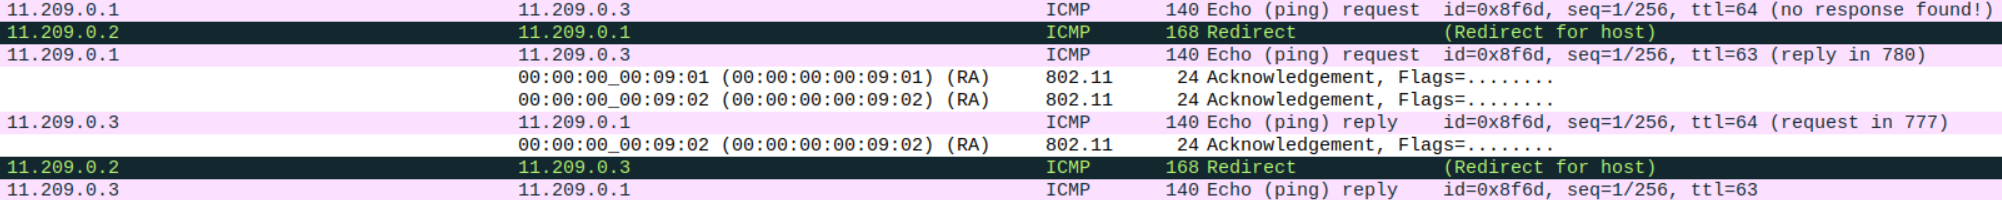
\includegraphics[width=\textwidth]{ej4.5}\\
	\end{figure}
\end{enumerate}
\end{document}
